\section{Auswertung}
\label{sec:Auswertung}

\subsection{Filterkurve des Selektiv-Verstärkers}

Die gemessenen Spannungen bei varrierten Frequenzen werden in der Tabelle \ref{tab:filter} dargestellt.
Die Güte Q wurde auf $Q = 20$ eingestellt.

\begin{table}[H]
    \centering
    \caption{Messwerte zur Bestimmung der Filterkurve.}
    \label{tab:filter}
    \begin{tabular}{c c}
        \toprule
        $\nu /kHz$ & $U / mV$ \\
        \midrule
        20    &  40   \\
        21    &  44   \\
        22    &  50   \\
        23    &  56   \\
        24    &  60   \\
        25    &  68   \\
        26    &  75   \\
        27    &  90   \\
        28    &  105  \\
        29    &  125  \\
        30    &  150  \\
        31    &  200  \\
        32    &  260  \\
        32.5  &  330  \\    
        33    &  440  \\
        33.3  &  500  \\ 
        33.5  &  600  \\
        33.8  &  700  \\
        34    &  800  \\
        34.3  &  1100  \\
        34.5  &  1300 \\
        34.8  &  1500 \\
        35    &  1400 \\
        35.3  &  1100 \\
        35.6  &  800 \\ 
        36    &  600 \\
        36.5  &  480 \\ 
        37    &  400 \\
        38    &  250 \\
        39    &  200 \\
        40    &  170 \\
        \bottomrule
    \end{tabular}
\end{table}

\noindent Die gemessenen Werte werden nun in \ref{fig:filter} dargestellt.

\begin{figure}[H]
    \centering
    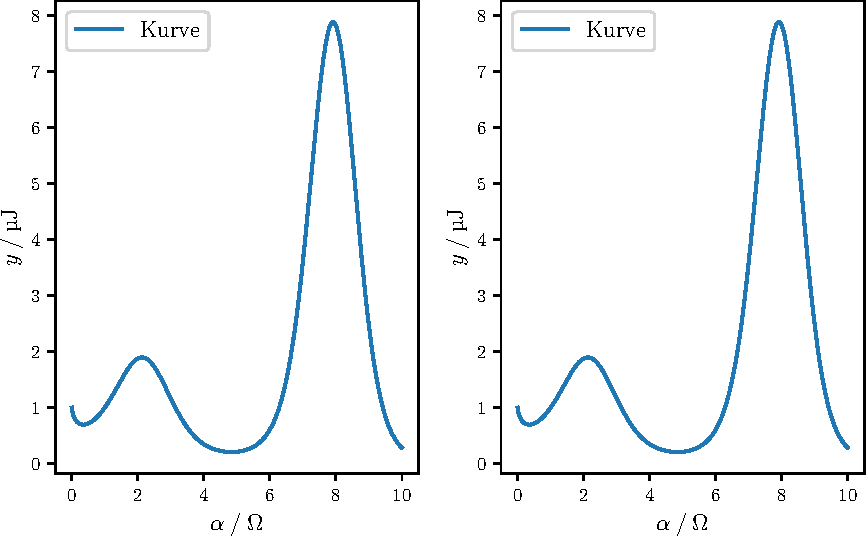
\includegraphics{build/plot.pdf}
    \caption{Filterkurve}
    \label{fig:filter}
\end{figure} 

\noindent Es ist zu erkennen, dass das Maximum der Ausgangsspannung bei einer Frequenz von $\nu = \qty{34.8}{kHz}$ liegt.

\subsection{Suszeptibilität von Seltener-Erd Elemente}

Da die Proben aus staubförmigen Material besteht und nicht aus einem Einkristall wird zuerst der reale Querschnitt $Q_\text{real}$ berechnet.
Mit diesem Wert werden die späteren Berechnungen als Q durchgeführt
Dafür wird die Formel 
\begin{equation}
    Q_\text{real} = \frac{M}{L \rho_w}
\end{equation}
verwendet.
Dabei beschreibt M die Masse der Probe, L die Länge der Probe und $\rho_w$ die Dichte des Materials als Einkristall.
Die berechneten Werte werden in der Tabell \ref{tab:Ergebnisse}dargestellt.

\noindent In den folgenden Tabellen werden die Messwerte dargestellt. Dabei bezeichnet $U_m$ die Spannung und $R_m$ der Widerstand, der gemessen wird, wenn die Proben sich
innerhalb der Spule befinden. 
Die Spannung und der Widerstand der gemessen wird, wenn sich keine Probe in der Spule befindet, werden als $U_o$ und $R_o$ bezeichntet.
Für die weiteren Berechnungen wird die Differenz der Spannnugen $\Delta U = U_m -U_o$ und des Widerstandes $\Delta R = R_m - R_o$ berechnet.
Diese Differenz wird ebenfalls in den Tabellen dargestellt.
Für die abgelesenen Meswerte für $R_m$ und $R_o$ gilt das 1 Ziffer $\widehat{=} 5 m \Omega$. 
Somit werden die Werte mit fünf multipliziert.

\begin{table}[H]
    \centering
    \caption{Messwerte für die Probe \ce{Nd2O3}}
    \label{tab:Nd}
    \begin{tabular}{c c c c c c}
        \toprule
        $U_m / mV$ & $U_o / 10^{-7}V$ & $R_m /m\Omega$ & $R_o /m\Omega$ & $\Delta U /mV$ & $\Delta R /m\Omega$ \\
        \midrule        
        10  & 5    & 3230  & 3295  & 9.99  &   65   \\ 
        12  & 1    & 3220  & 3305  & 11.99  &  85    \\ 
        19  & 1.5  & 3230  & 3340  & 18.99  &  110    \\ 
        \bottomrule
    \end{tabular}
\end{table}

\begin{table}[H]
    \centering
    \caption{Messwerte für die Probe \ce{Dy2O3}.}
    \label{tab:Dy}
    \begin{tabular}{c c c c c c}
        \toprule
        $U_m / mV$ & $U_o / 10^{-7}V$ & $R_m /m\Omega$ & $R_o /m\Omega$ & $\Delta U /mV$ & $\Delta R /m\Omega$ \\
        \midrule        
        270  & 2  & 1830  &  3335 & 269.99  &  1505    \\ 
        270  & 4  & 1800  &  3320 & 269.99  &  1520    \\ 
        270  & 3  & 1850  &  3325 & 269.99  &  1475    \\ 
        \bottomrule
    \end{tabular}
\end{table}

\begin{table}[H]
    \centering
    \caption{Messwerte für die Probe \ce{Gd2O3}.}
    \label{tab:Gd}
    \begin{tabular}{c c c c c c}
        \toprule
        $U_m / mV$ & $U_o / 10^{-7}V$ & $R_m /m\Omega$ & $R_o /m\Omega$ & $\Delta U /mV$ & $\Delta R /m\Omega$ \\
        \midrule        
        60  & 3  & 2705  & 3315  & 59.99  & 610     \\ 
        60  & 3  & 2700  & 3315  & 59.99  & 630     \\ 
        65  & 3  & 2700  & 3325  & 64.99  & 645     \\ 
        \bottomrule
    \end{tabular}
\end{table}
\noindent Die Werte werden nun zur weiteren Berechnung gemittelt.
Die gemittelten Werte sind in der Tabelle \ref{tab:Ergebnisse} zu finden.
Zur Berechnung der Suszeptibilität $\chi_R$ wird die Formel \ref{eq:chiR} verwendet.
Dabei beträgt $R_3 = \SI{998}{\ohm}$ und der Querschnitt der Spule $F=\SI{86.6e-6}{\meter\squared}$.
Zudem wird auch die Suszeptibilität $\chi_U$ mithilfe der Formel \ref{eq:chiU} berechnet.
Dabei beträgt die Speisespannung $U_\text{Sp} = \qty{1.5}{V}$.
Die berechneten Werte werden in der Tabelle \ref{tab:Susz} dargestellt.

\begin{table}[H]
    \centering
    \caption{Berechnete Werte.}
    \label{tab:Ergebnisse}
    \begin{tabular}{c c c c c c c c}
        \toprule
        $Stoff$ & $M / g$ & $L / cm$ & $Q_\text{real} /10^{-6}m^2 $ & $U_\text{mittel} /mV$ & $R_\text{mittel} / m\Omega$ \\
        \midrule        
        \ce{Nd2O3}  & 7.66  & 18    & 5.87   & 13.65  & 87   \\
        \ce{Dy2O3}  & 15.1  & 17.5  & 11.06  & 269.99 & 1500 \\ 
        \ce{Gd2O3}  & 10.2  & 17.5  & 7.87   & 61.70  & 628  \\
        \bottomrule
    \end{tabular}
\end{table}

\begin{table}[H]
    \centering
    \caption{Berechnete Suszeptibilität.}
    \label{tab:Susz}
    \begin{tabular}{c c c}
        \toprule
        $Stoff$ &  $\chi_U$ & $\chi_R$ \\
        \midrule        
        \ce{Nd2O3}  & 0.0054 \pm 0.0015  & 0.0026 \pm 0.0005   \\ 
        \ce{Dy2O3}  & 0.0563 \pm 0.000000017  & 0.0235 \pm 0.00029   \\ 
        \ce{Gd2O3}  & 0.0181 \pm 0.0007  &  0.0138 \pm 0.0007  \\ 
        \bottomrule
    \end{tabular}
\end{table}